\documentclass{article}
\usepackage{graphicx} % Required for inserting images
\usepackage[a4paper, margin=1.2in]{geometry}
\usepackage{amsmath}
\usepackage{amssymb}
\usepackage{float}

%\usepackage{listings}

\usepackage{hyperref}

\title{Exploring Aliasing and the Sampling Theorem} %\\\large\textit{Approximation Part 2 Assignment}}
\author{Margherita Tonon}
\date{April 2025}

\begin{document}

\maketitle

\section{Introduction}
In signal processing, computers analyze and process discrete time signals. 
However, most signals of interest are continuous time signals, as these are the signals most commonly found in nature -- e.g. sound waves.
We therefore use sampling, allowing us to convert a continuous-time signal into a discrete signal that a computer is able to process.
Nonetheless, one of the factors determining the accuracy in the information content of sampled signals is the sampling rate. %not sure if i should mention quantization, because i dont mention it at all ever.
Given that the Shannon-Nyquist theorem, a condition relating to the sampling rate, is met, a signal can be perfectly recovered from its sampled signal. 
However, if this condition is not met, a signal can no longer be perfectly recovered due to a phenomenon named aliasing [1].
Here, we will explore the process of recovering a sampled signal, looking at different sampling rates that meet and do not meet the conditions for perfect signal recovery.

%introduction sentence, context, motivation

\section{Background}
In signal processing, signals are commonly categorized as analog signals and digital signals.
An analog signal refers to a signal that varies continuously over time. 
The complexity of analog signal processing, their susceptibility to noise and signal degradation over time, as well as their limited reproductibility and scalability makes them inconvenient to work with in practice. 
Therefore, digital signals are used -- signals that vary discretely over time and can take only a finite number of distinct values.
%mention advantages of digital signals?

Sampling refers to the process of converting an analog signal into a digital signal. If we let $x(t)$ be a continuous time signal, the sampled signal $x[n]$ is defined as
\begin{center}
    \begin{math}
        x[n] = x(nT_s)
    \end{math}  
\end{center}
where $n$ represents discrete time sampling points and $T_s$ represents the sampling period, such that the sampling frequency $f_s = \frac{1}{T_s}$.

Sampling can also be represented as 
\begin{center}
    \begin{math}
        x_s(t) = x(t) \displaystyle\sum_{n=-\infty}^{\infty} \delta (t-nT_s)
    \end{math}  
\end{center}
where $x_s(t)$ is the sampled points, and $\delta$ is the Dirac Delta distribution, taking value 1 if $t=nT_s$, and 0 otherwise.
Therefore, it is clear that when $t=nT_s$, $x_s(t) = x(t)$; otherwise, $x_s(t) = 0$. 

In practice, sampling allows us to discretize a continuous input, facilitating the handling of signals. After sampling is done, it is natural that the signal must be reconstructed in order to recover the original (time continuous) signal.
However, recovery is not always perfect -- the Shannon-Nyquist condition must be met.
%something along the lines of: the key issue is what must the sampling frequency be in order for a signal to be perfectly reconstructed and recovered?

The Shannon-Nyquist theorem states that a signal can be perfectly reconstructed if the sampling frequency is greater than two times the maximum frequency $B$ of the continuous signal:
\begin{center}
    \begin{math}
        f_s > 2B
    \end{math}  
\end{center}
For example, if we consider a sine wave with frequency 2 Hertz (Hz), $\sin(2\pi \cdot 2 \cdot t)$, once sampled it can be perfectly reconstructed if the sampling frequency is greater than 4 Hz.

%do i explain quantization here?

In the time domain, a sampled signal looks like discrete spikes (Figure 1). 
%\begin{figure} %TODO: not sure if i should change this plot so that it has the og signal on the left and the sampled signal on the right, but maybe make it above shannon hyquist so that ppl actually get a sense of what happens
%    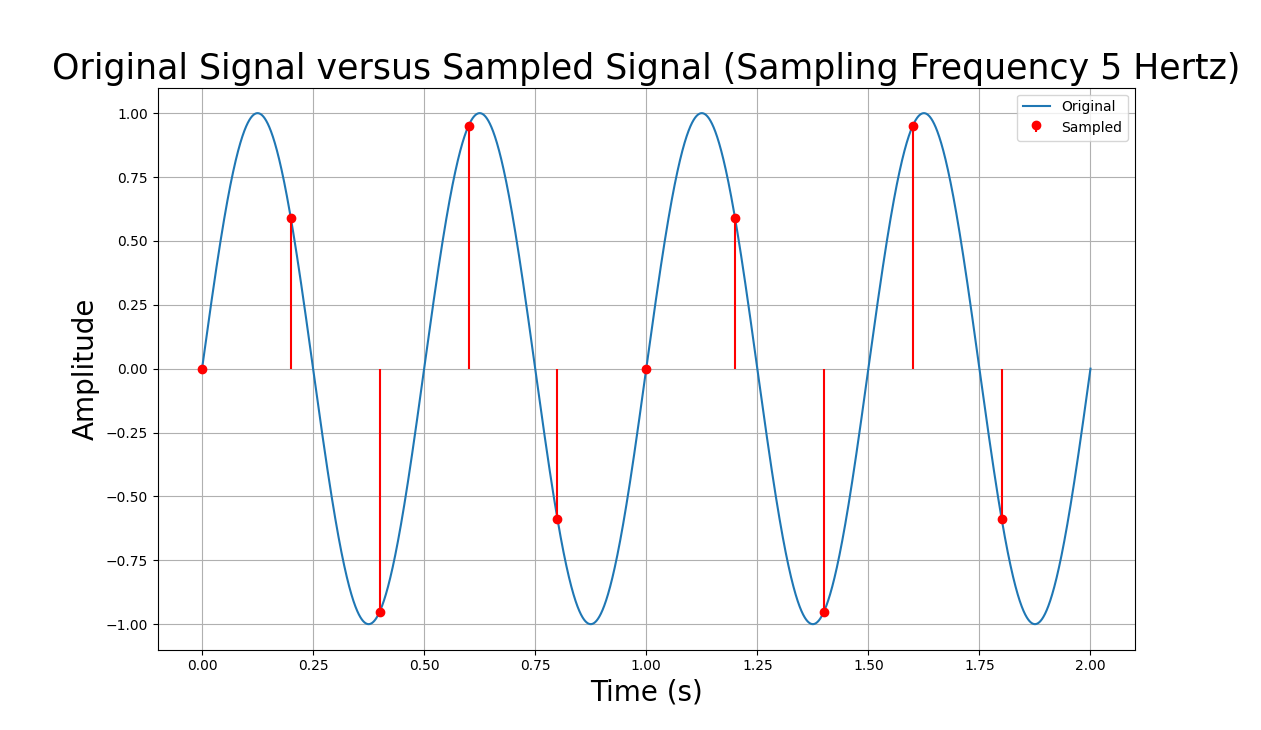
\includegraphics[width=\linewidth]{images/ogvssampled_BIG.png}
%    \caption{Representation of sampling of $\sin(4\pi t)$ in the time domain, sampled at a frequency of 5 Hertz}
%    \label{fig:grid}
%\end{figure}

\begin{figure}[H]
    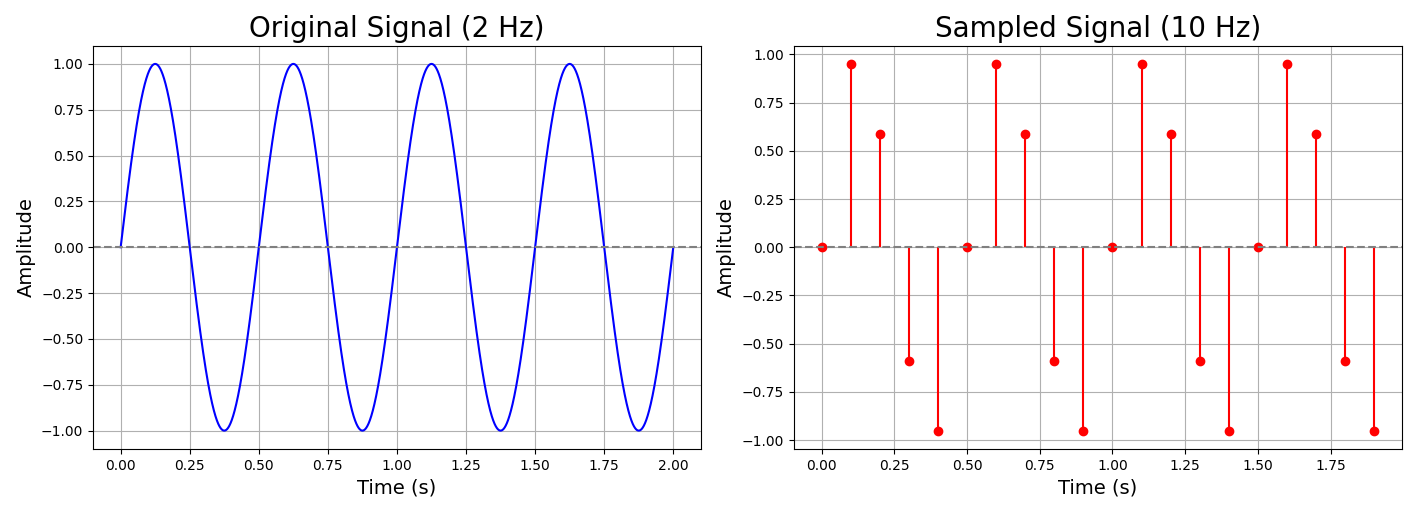
\includegraphics[width=\linewidth]{images/leftright_ogsampled.png}
    \caption{Representation of sampling of $\sin(4\pi t)$ in the time domain, sampled at a frequency of 10 Hz.}
    \label{fig:enter-label}
\end{figure}
The Fourier Transform, defined as
\begin{center}
    \begin{math}
       X(f) = \displaystyle \int_{-\infty}^{\infty} x(t)e^{-i2\pi ft}\, dt
    \end{math}
\end{center}
allows us to transition from the time domain into the frequency domain. In order to visualize what sampling looks like in the frequency domain, we make use of the Inverse Convolution Theorem.

The Inverse Convolution Theorem states that if we have two functions $x(t)$ and $h(t)$ whose Fourier Transforms $\mathcal{F}(x(t))$ and $\mathcal{F}(h(t))$ are absolutely integrable in the frequency domain,
then 
\begin{center}
    \begin{math}
        \mathcal{F}^{-1} \left(X(f) * H(f) \right) = x(t) \cdot h(t)
    \end{math}  
\end{center}
where $*$ denotes the convolution operator. 
Consequently, if $x(t)$ and $h(t)$ are absolutely integrable and the Fourier Transform of their product exists,
\begin{center}
    \begin{math}
        X(f) * H(f) = \mathcal{F}\left(x(t) \cdot h(t)\right)
    \end{math}  
\end{center}
%if $x(t)$ and $h(t)$ are two absolutely integrable functions in $\mathcal{L}^1(\mathbb{R})$, and if their Fourier transforms $\mathcal{F}(x(t))$ and $\mathcal{F}(h(t))$ exist and are well defined,

Therefore, because we can express sampling as $x_s(t) = x(t) \cdot \displaystyle\sum_{n=-\infty}^{\infty} \delta (t-nT_s)$ in the time domain, the Inverse Convolution Theorem tells us that %i dont know if here its convolution thm or inverse convolution thm
\begin{center}
    \begin{math}
        \mathcal{F}\left(x(t) \cdot \displaystyle\sum_{n=-\infty}^{\infty} \delta (t-nT_s)\right) = \mathcal{F}(x(t)) * \mathcal{F}\left(\displaystyle \sum_{-\infty}^{\infty} \delta (t-nT_s) \right)
    \end{math}  
\end{center}

To visualize sampling in the frequency domain we must therefore convolve the Fourier Transform of the input signal with the Fourier Transform of $\displaystyle\sum_{n=-\infty}^{\infty} \delta (t-nT_s)$, known as the Dirac comb.
Using properties of the Fourier Transform, Dirac Delta distribution, Fubini's Theorem of exchanging the order of integration and summation, 
and the Poisson summation formula, 
we obtain that 
\begin{center}
    \begin{math}
        \mathcal{F}\left(\displaystyle\sum_{-\infty}^{\infty} \delta (t-nT_s)\right) = \frac{1}{T_s} \displaystyle\sum_{k = -\infty}^{\infty} \delta \left( f - \frac{k}{T_s} \right)
    \end{math}  
\end{center}
We therefore have
\begin{center}
    \begin{math}
        \mathcal{F}(x(t)) * \mathcal{F}\left(\displaystyle \sum_{n=-\infty}^{\infty} \delta (t-nT_s) \right) = X(f) * \frac{1}{T_s}\displaystyle \sum_{k = -\infty}^{\infty} \delta \left( f - \frac{k}{T_s} \right)
    \end{math}  
\end{center}
Convolution of a function with a delta function shifts the function by the offset/position of the delta function, and therefore 
\begin{center}
    \begin{math}
        \mathcal{F}(x(t)) * \mathcal{F}\left(\displaystyle \sum_{n=-\infty}^{\infty} \delta (t-nT_s) \right) 
        = 
        \frac{1}{T_s} \displaystyle\sum_{k=-\infty}^{\infty}X\left(f - \frac{k}{T_s} \right)
    \end{math}  
\end{center}

We can therefore observe how the representation of a sampled signal in the frequency domain is simply the Fourier Transform of the signal, duplicated and shifted to multiples of the sampling frequency.

When recovering the original signal, we assume that the Shannon-Nyquist condition is met. 
Because $f_s > 2B$, the original signal has to be contained within the range of frequencies $\frac{-f_s}{2}$ and $\frac{f_s}{2}$, as $\frac{-f_s}{2} < -B$ and  $\frac{f_s}{2} > B$. 
Because the frequency domain representation of a signal has the frequency of the signal as well as the negative frequency of the signal, we only need to consider the positive frequencies: $0$ to $\frac{f_s}{2}$ Hz. %todo: rephrase
We therefore apply a low pass filter with cutoff frequency $f_l = \frac{f_s}{2} = \frac{1}{2T}$.
In the frequency domain, we would multiply this low pass filter with the sampled signal, and then perform an inverse Fourier Transform on the signal.

Nonetheless, the frequency domain representation of the sampled signal and the low pass filter highlight the need for the Shannon-Nyquist theorem.
When filtering a sampled signal, we effectively only see and select the frequencies between $\frac{-f_s}{2}$ to $\frac{f_s}{2}$.
If $f_s = 2B$, this range becomes $[-B, B]$, and therefore all of the frequency components of the original signal are included.
However, when $f_s < 2B$, the filter will select frequencies on a range $[-a, a]$, where $a < B$. Clearly, $B$ is not included within this range and we end up missing part of the original spectrum.
We recall that sampling in the frequency domain replicates the original spectrum $X(f)$ at every integer multiple of $f_s$.
If $f_s$ is too small, some copied frequencies will shift into in the interval $\left[\frac{-f_s}{2}, \frac{f_s}{2}\right]$ -- this is known as folding.
When filtering, these folded frequencies will be wrongly interpreted as the original signal's frequency, and therefore the original signal will not be reconstructed correctly.
The process of different frequency components becoming indistinguishable in the sampled signal due to overlapping spectra is known as aliasing.
On the other hand, if $f_s > 2B$, the range $\left[\frac{-f_s}{2}, \frac{f_s}{2}\right]$ fully contains $\left[-B, B \right]$. 
Because $f_s$ is sufficiently large, the shifted copies will not land inside $\left[\frac{-f_s}{2}, \frac{f_s}{2}\right]$, and the original signal can be reconstructed perfectly.

%When $f_s < 2B$, the filter will select frequencies between a value larger than $-B$ to a value smaller than $B$. Clearly, $B$ is not contained within this range. 
%Recalling that sampling in the frequency domain looks like copying and shifting the Fourier transform of the original signal, a small sampling frequency will cause some copied frequencies to land within the range $[\frac{-f_s}{2}, \frac{f_s}{2}]$ -- this is known as folding.
%When filtering, these folded frequencies will be wrongly interpreted as the original signal's frequency, and therefore the original signal will not be reconstructed correctly.
%The process of different frequency components becoming indistinguishable in the sampled signal due to overlapping spectra is known as aliasing.
%If $f_s > 2B$, the largest frequency component of the original signal will be in the selected frequency range, as the ranges will go from a value less than $B$ to a value greater than $B$.
%Folding will not occur here as the process of copying and shifting the frequencies occurs at larger intervals, meaning the copied frequencies are more spread out, and the shifted copies of the spectrum do not land inside $[\frac{-f_s}{2}, \frac{f_s}{2}]$.

%Nonetheless, the frequency domain representation of the sampled signal highlights the need for the Shannon-Nyquist theorem. %maybe not "need" but like utility/usefulness or something
%When our sampling frequency is sufficiently large, the process of copying and shifting the frequencies occurs at larger intervals, meaning the copied frequencies are more spread out. 
%As a result, it is possible to apply an ideal filter to recover the original frequencies. 
%However, if the sampling frequency decreases, the interval between frequencies is not as large and they may overlap. It is therefore no longer possible to apply an ideal filter to recover the original frequencies, as the original signal and the duplicated frequencies overlap and interfere with each other.
%This phenomenon is known as aliasing: the act of different frequency components becoming indistinguishable in the sampled signal due to overlapping spectra. %maybe use a diff definition cause this is rly similar to the one on the slides
%As long as we set $f_s > 2B$, however, the signal can be perfectly recovered. 

%maybe give an example of aliasing happening, like the one we saw in class?

%some context into the problem, theory
%overview of what sampling is, why its used!! important to say why sampling
%what happens when we sample?
%the problem of reconstruction and the need for sufficiently high sampling frequencies

\section{Implementation}
%TODO: insert code snippets and change the function names to actual code block writing
%explanation of code
%the theory behind the sinc function bc thats what we implement when we have been talking about ideal band pass filter the entire time
%here dont put all of the different frequencies because we do that in the discussion

%maybe like one sentence of what the sampling process consists of

To implement the process of sampling in Python, I begin by defining a function \verb|generate_signal| which generates a continuous time signal.
If the parameter \verb|signal_type| is set to \verb|"single"|, a sine wave of desired frequency is created.
If this parameteris set to \verb|"multiple"|, a sine wave of desired frequency is added to a sine wave with half of the desired frequency. 
%\begin{lstlisting}[language = Python]
%\end{lstlisting}
%insert code block here
Here, I simply create a time array with $5000t_e$ elements, where $t_e$ is the duration in seconds of the signal, 
and then apply the sine function with the given frequency to the $5000 t_e$ time values. 
Users can set the \verb|plot| parameter to \verb|True| if they wish a plot of the original continuous-time signal to be displayed.

Next, I define the \verb|sample_signal| function, which samples the continuous signal at a specified sampling frequency.
%code block of sample_signal
In this code block, I create a new time array \verb|t_sampled| for the sampled signal using the sampling period, representing the new set of discrete time points. 
Next, I use \verb|np.interp| to perform the sampling of the original signal \verb|x| at the time points in the \verb|t_sampled| array.
Users can set \verb|plot_one| to \verb|True| if they wish to visualize the original signal together with the sampled points, \verb|plot_two| to \verb|True| if they wish to just visualize the sampled points, and \verb|plot_three| to \verb|True| to visualize both plots side by side.

Thirdly, I create the \verb|sampled_fourier_transform| function, which takes as inputs the sampled amplitudes, the sampling frequency, and the number of times to repeat the spectrum ($k$), 
and performs the Fast Fourier Transform of the sampled amplitudes using the \verb|scipy| module [2].
The Fourier Transform integrates a signal over all time (from $-\infty$ to $+\infty$) and requires a signal to be continuous. 
However, in many practical situations, such as our current scenario, we work with finite and discrete signals. 
The Discrete Fourier Transform allows us to numerically compute the Fourier Transform for a finite time interval, 
and the Fast Fourier Transform is a way of computing the Discrete Fourier Transform in a more computationally efficient way. 
Therefore, in the \verb|sampled_fourier_transform| function, \verb|yf| is a complex array representing the sampled signal \verb|x_sampled| in the frequency domain, 
and \verb|xf| is the frequency values, in Hertz, that each element in \verb|yf| corresponds to. %i think that maybe it has something to do with ck of the DFT? not sure tho
If \verb|plot| parameter is set to \verb|True|, a plot of the frequencies of the sampled signal in the frequency domain is shown.
%code block

Finally, I define the \verb|reconstruction| function, which reconstructs the original signal from the sampled signal.
This function takes as inputs the array of the amplitudes of the sampled signal \verb|x_sampled| and the time array of the sampled signal \verb|t_sampled|.
If users wish to plot the reconstructed signal together with the original signal, they must set the \verb|plot| parameter to \verb|True| and provide the original signal \verb|x_continuous| as well as the continuous time array \verb|t_s|.
%code block here

In the code, I reconstruct the signal in the time domain using the sinc function.
Previously, we mentioned that we must apply a low pass filter with cutoff frequency $f_l = \frac{f_s}{2}$ to recover the signal.
The convolution theorem states that if $x(t)$ and $h(t)$ are two absolutely integrable functions in $\mathcal{L}^1$, and if their Fourier transforms $X(f) = \mathcal{F}(x(t))$ and $H(f) = \mathcal{F}(h(t))$ exist and are well defined,
\begin{center}
    \begin{math}
       \displaystyle \mathcal{F}\{ x(t) * h(t) \} = X(f) \cdot H(f)
    \end{math}
\end{center}
We therefore can convolve the time-domain representation of the lowpass filter with the sampled signal, and we will obtain the filtered signal.

The low pass filter has an impulse response defined as
\begin{center}
    \begin{math}
        h(t) = \displaystyle \frac{1}{T} \; \text{sinc} \left( \frac{t}{T} \right)
    \end{math}
\end{center}
where $\text{sinc}(x) = \frac{\sin(\pi x)}{\pi x}$.

Recalling that our sampled signal is $x(nT)$, their convolution is
\begin{center}
    \begin{math}
        \displaystyle \int_{-\infty}^{\infty} \displaystyle \left [ \sum_{n=-\infty}^{\infty} x(nT) \delta (\tau - nT) \displaystyle \right ] \cdot h(t - \tau) d\tau
    \end{math}
\end{center}

After some simplifications, we obtain that the recovered signal can be found using
\begin{center}
    \begin{math}
        \displaystyle \sum_{n = -\infty}^{\infty} x(nT) \cdot \text{sinc} \left( \frac{t-nT}{T} \right)
    \end{math}
\end{center}
which is the approach implemented in the \verb|reconstruction| function.

However, because it is not possible to compute an infinite sum numerically, I must loop over a finite number of iterations. Mathematically, this looks like
\begin{center}
    \begin{math}
        x(t) \approx \displaystyle\sum_{n}^{} x[n]\, \text{sinc}\left( F_st - n \right)
    \end{math}  
\end{center}
where $F_s = 1/T$ and $x[n]$ is the value of the signal at the $n$-th sampling point.

\section{Discussion}
%results of code
%different initial frequencies, different sampling frequencies based on shannon nyquist thm

%we see that we have not exactly the same reconstruction and original but this is bc of: Finite number of samples, Numerical approximations (e.g., np.sinc is not truly ideal), Edge effects due to time-domain boundaries --> CHECK WHAT THESE MEAN. could it also be related to quantization?

We begin by observing a continuous time signal: $x(t) = \sin(2\pi\cdot5t) + \sin(\pi\cdot5t)$ (Figure 2). 
\begin{figure}[H]
    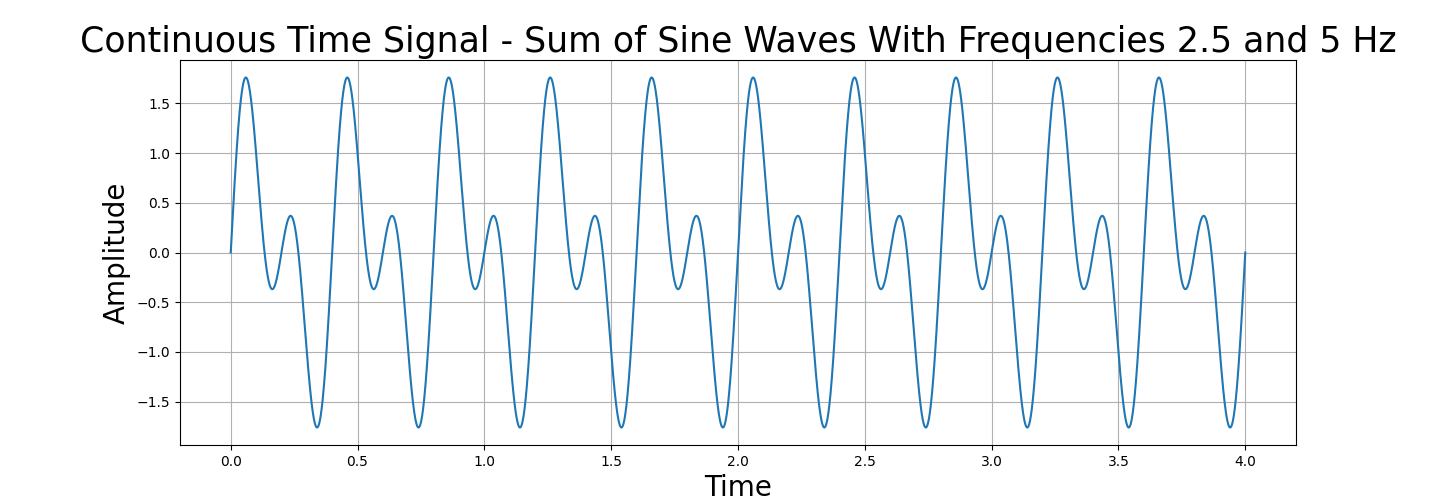
\includegraphics[width=\linewidth]{images/ogtimedom.png}
    \caption{Continuous time signal $x(t) = \sin(2\pi\cdot5t) + \sin(\pi\cdot5t)$.}
    \label{fig:enter-label}
\end{figure}
The highest frequency component of this signal is $B = 5$. 
According to the Shannon-Nyquist theorem, if we sample the signal at a frequency greater than $2\cdot 5 = 10$ Hz, we can perfectly reconstruct the signal.
Sampling the wave with sampling frequencies of 12 Hz (above the Shannon-Nyquist threshold) and 7 Hz (below the Shannon-Nyquist threshold) is seen in Figure 3.

\begin{figure}[H]
    \centering
    \begin{minipage}{0.8\textwidth}
        \centering
        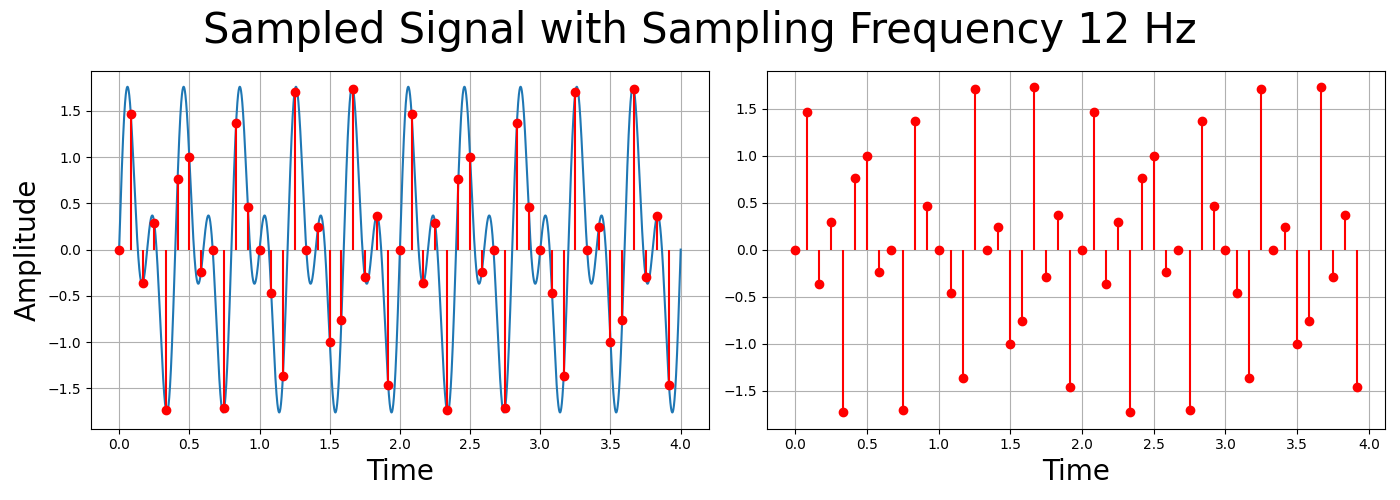
\includegraphics[width=\linewidth]{images/new_sampled_12hz.png}
        \\[0.5em] 
    \end{minipage}
    
    \begin{minipage}{0.8\textwidth}
        \centering
        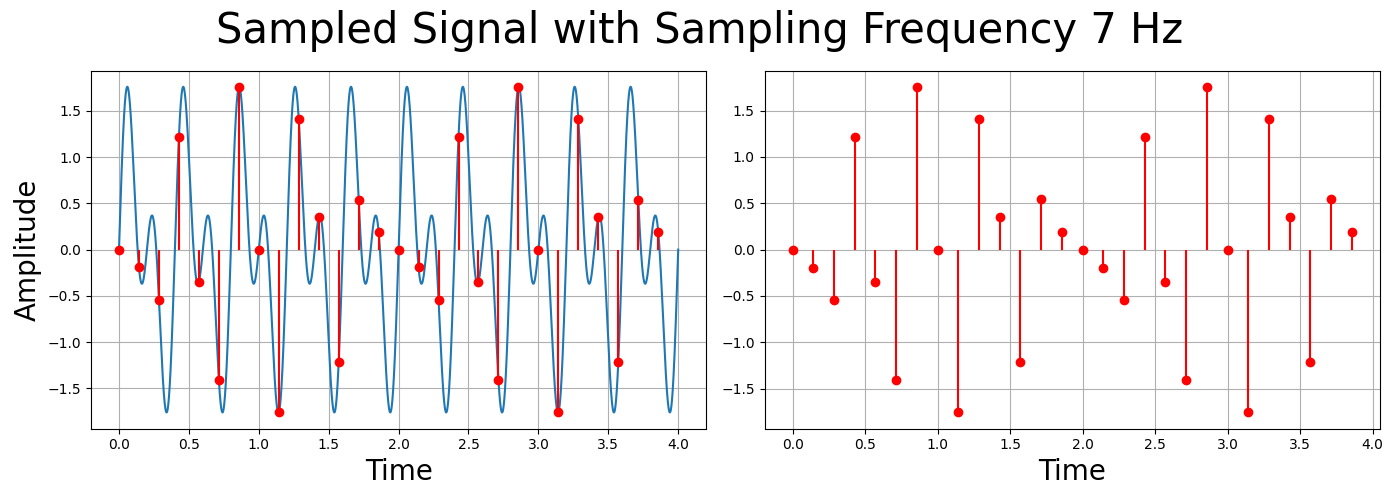
\includegraphics[width=\linewidth]{images/new_sampled_7hz.png}
    \end{minipage}
    
    \caption{Visualization of the sampling a continuous time signal with a sampling frequency 12 Hz (top) and 7 Hz (bottom). 
    The original signal is in blue on the left plots, and the red spikes are the sampled amplitudes.}
\end{figure}
%\begin{figure}[H]
%    \centering
%    \begin{minipage}{0.8\textwidth}
%        \centering
%        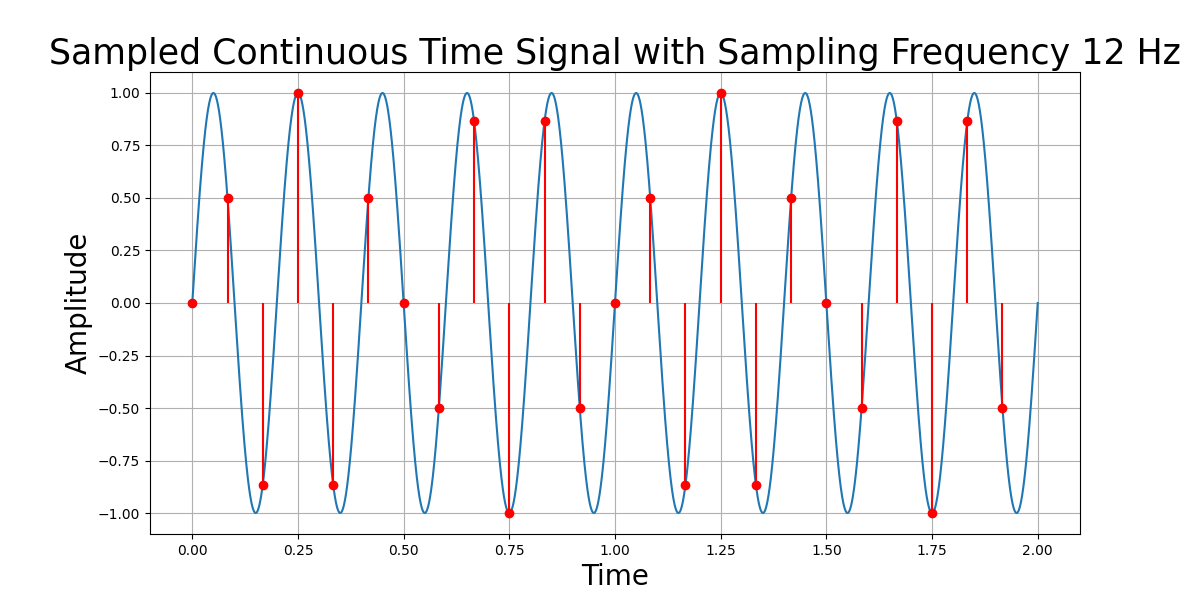
\includegraphics[width=\linewidth]{images/sampled_12hz_1.png}
%        \\[0.5em] % optional spacing between rows
%    \end{minipage}
    
%    \begin{minipage}{0.8\textwidth}
%        \centering
%        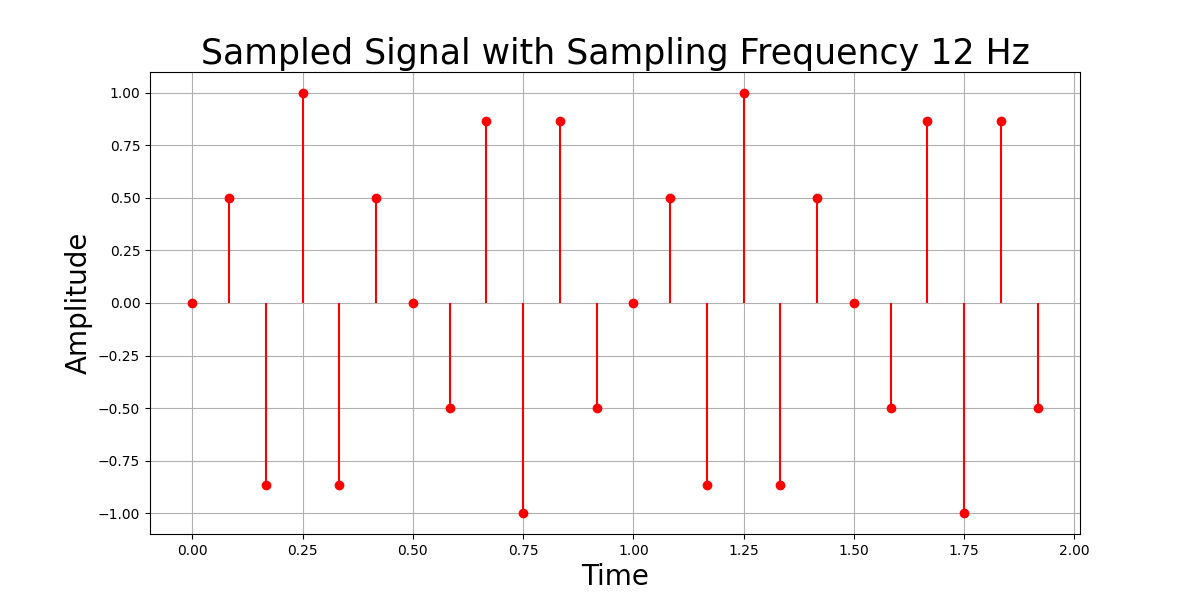
\includegraphics[width=\linewidth]{images/sampled_12hz_2.png}
%    \end{minipage}
    
%    \caption{Visualization of the sampling a continuous time signal with a sampling frequency 12 Hz.}
%\end{figure}

%\begin{figure}[H]
%    \centering
%   \begin{minipage}{0.8\textwidth}
%        \centering
%        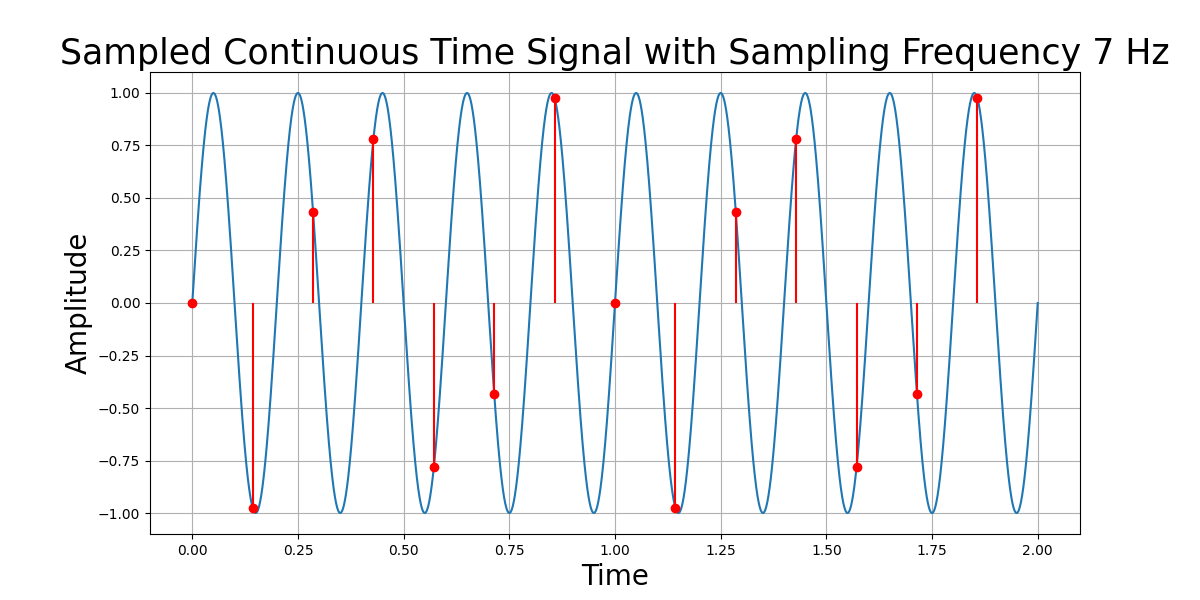
\includegraphics[width=\linewidth]{images/sampled_7hz_1.png}
%        \\[0.5em] % optional spacing between rows
%    \end{minipage}
    
%    \begin{minipage}{0.8\textwidth}
%        \centering
%        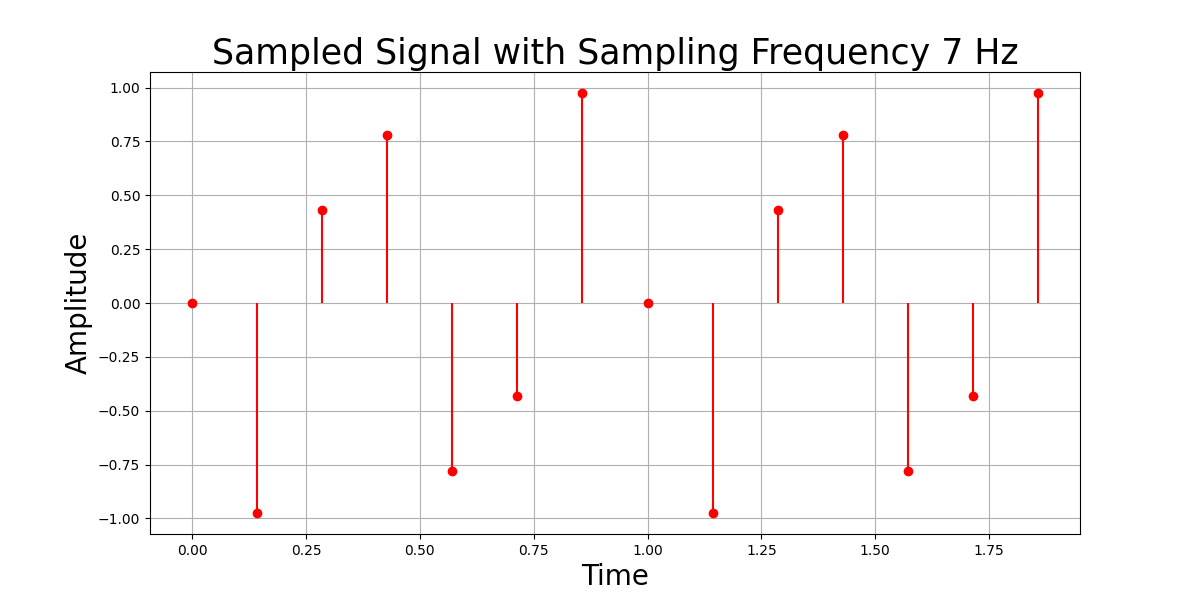
\includegraphics[width=\linewidth]{images/sampled_7hz_2.png}
%    \end{minipage}
    
%    \caption{Visualization of the sampling a continuous time signal with a sampling frequency 7 Hz.}
%\end{figure}

As expected, the time domain representation of the signal sampled at 12 Hz has more spikes than the signal sampled at 7 Hz, as a higher sampling frequency implies a signal is sampled more times within a given time interval.
%this is the expected behaviour as a sampling frequency of 12 Hz 
%this is the expected behaviour as 12 Hz being a higher sampling frequency than 7 Hz means that the signal is sampled more times across a given time interval (here being 2 seconds). 

In the frequency domain, the original continuous time signal looks like four spikes at $5$, $-5$, $2.5$, and $-2.5$ Hz (Figure 4).
\begin{figure}[H]
    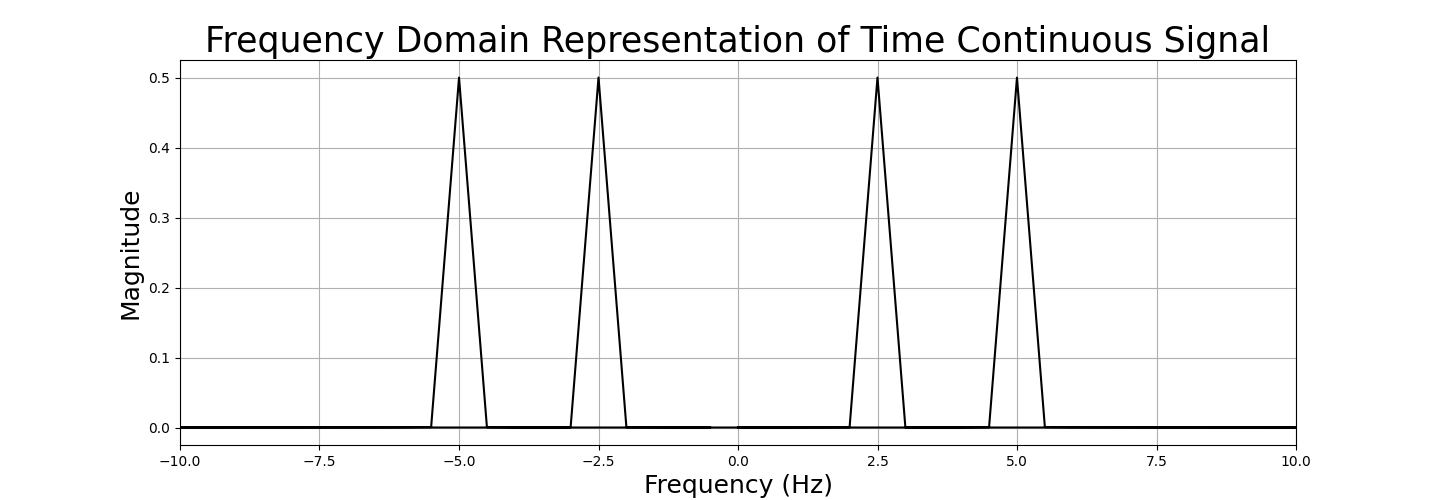
\includegraphics[width=\linewidth]{images/freqdom_timecont_black.png}
    \caption{Frequency domain representation of the continuous time signal.}
    \label{fig:enter-label}
\end{figure}

Figure 5 shows the frequency domain representation of the signal sampled at 12 Hz together with the reconstructed signal. 

\begin{figure}[H]
    \centering
    \begin{minipage}{\textwidth}
        \centering
        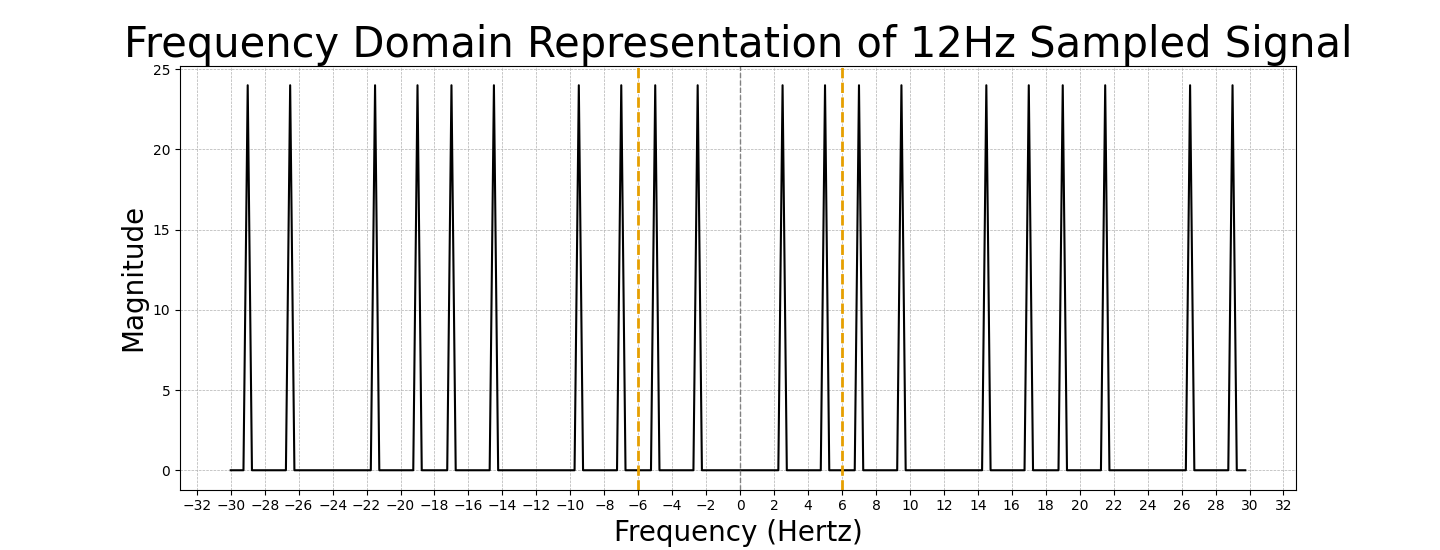
\includegraphics[width=\linewidth]{images/orange_freqdom_12hz.png}
        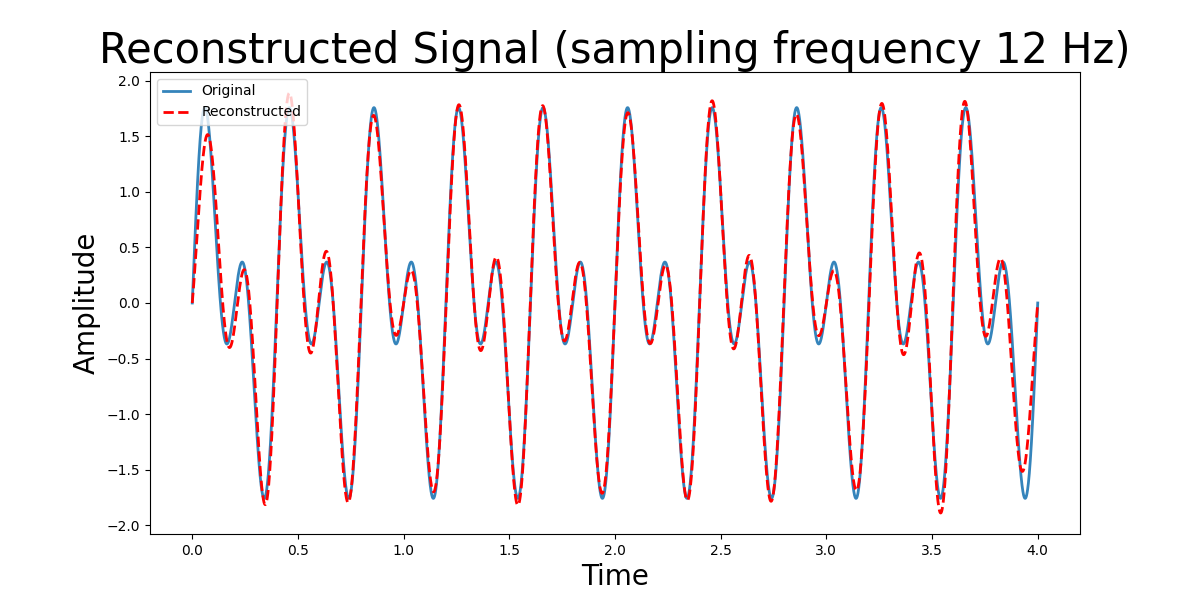
\includegraphics[width=\linewidth]{images/ogcolors_reconstructed_12hz.png}
        \\[0.5em] 
    \end{minipage}
    \caption{Frequency domain representation of sampled signal at 12 Hz (top), and the reconstructed signal (bottom). 
    The orange dotted lines represent the low pass filter cutoff frequencies $\pm \frac{f_s}{2}$.}
\end{figure}
Here, the sampling frequency is above the Shannon-Nyquist threshold, and we can see that both of the frequency components of the original signal (2.5 and 5 Hz) are contained within the filtering bound -- which in this case is at $\frac{12}{2}=6$ Hz. 
Because sampling replicates the original spectrum $X(f)$ at every integer multiple of $f_s$, we do not see any frequencies fold when $f_s > 2B$ as the integer multiples are larger than the bandwidth of the original signal.
Therefore, when the low pass filter is applied, the signal's original frequencies will be recovered and the signal will be perfectly reconstructed, as can be seen in the bottom plot of Figure 5.
The slight inconsistencies are due to numerical errors in truncating infinite sums.

However, when the sampling frequency is below the Shannon-Nyquist threshold, we can clearly see aliasing occur.
Figure 6 shows the frequency domain representation of the signal sampled at 7 Hz together with the reconstructed signal.

\begin{figure}[H]
    \centering
    \begin{minipage}{\textwidth}
        \centering
        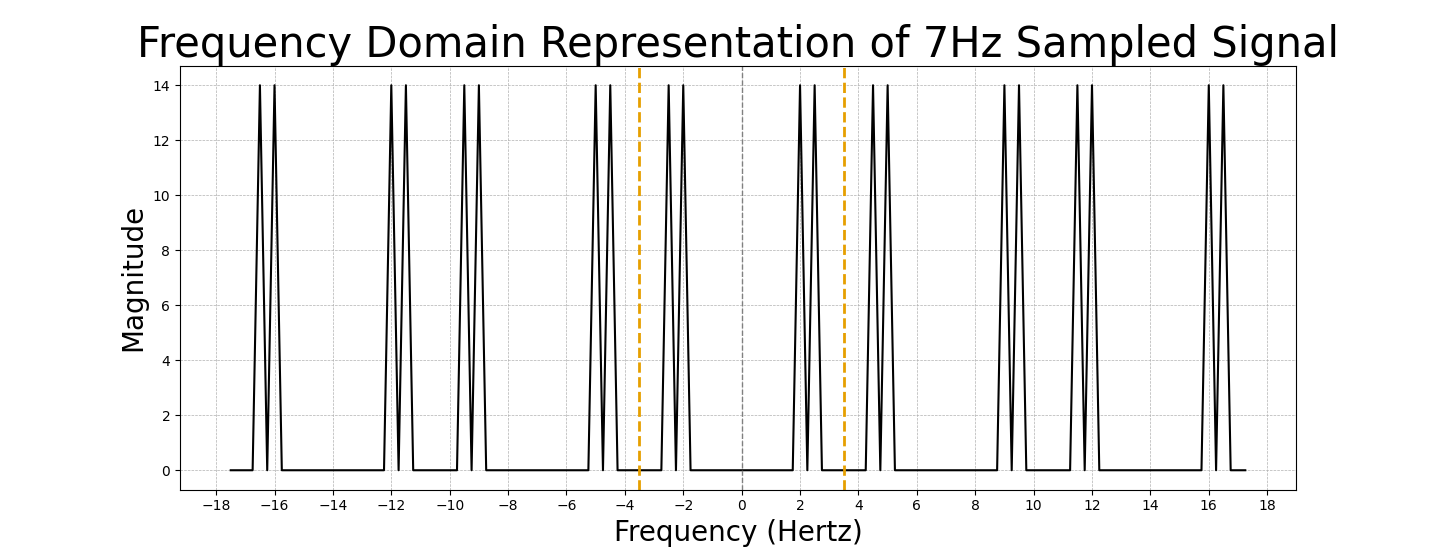
\includegraphics[width=\linewidth]{images/orange_freqdom_7hz.png}
        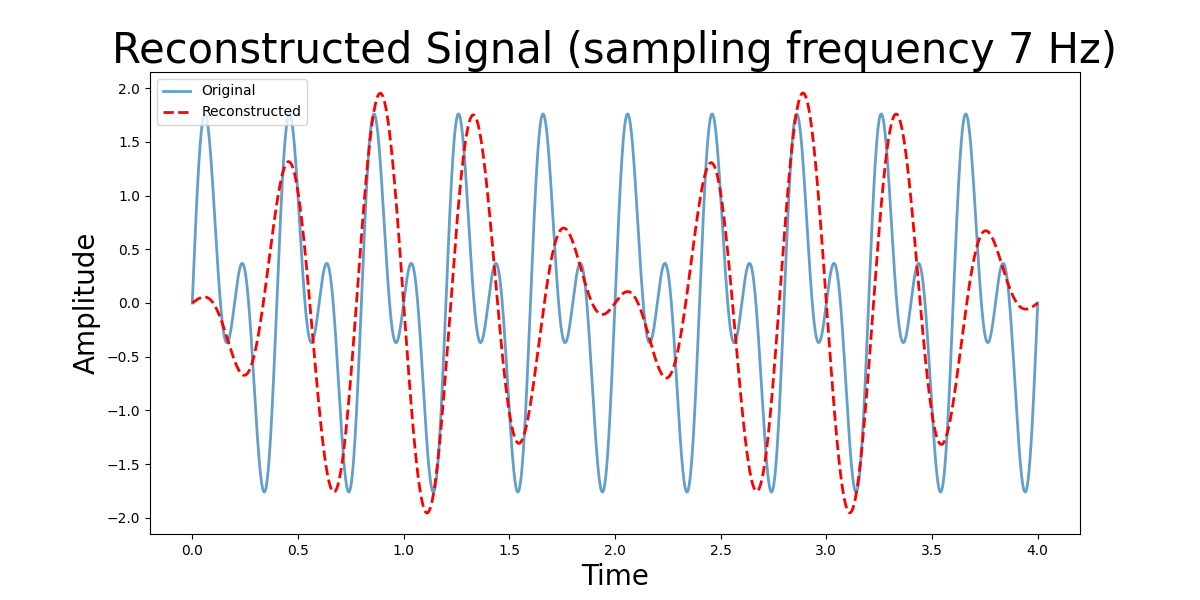
\includegraphics[width=\linewidth]{images/ogcolors_reconstructed_7hz.png}
        \\[0.5em] 
    \end{minipage}
    \caption{Frequency domain representation of sampled signal at 7 Hz (top), and the reconstructed signal (bottom). 
    The orange dotted lines represent the low pass filter cutoff frequencies $\pm \frac{f_s}{2}$.}
\end{figure}

In the frequency domain plot (top), we can see that the low pass filter bounds are $\pm 3$ Hz.
This means the 5 Hz frequency component from the original signal lies outside the filter range and is therefore not captured.
Moreover, we also observe folding happening. The $5$ Hz frequency is folded back on $f_s = 7$ Hz, landing on $-2$ Hz. 
Similarly, the $-5$ Hz frequency also folds back and lands on $-5+7=2$ Hz. This is why we see the $\pm 2$ Hz frequencies within the filtering window.
When the low pass filter with cutoff frequency $\frac{f_S}{2} = 3.5$ Hz is applied, it captures the 2 and 2.5 Hz frequencies, reconstructing an incorrect signal, as seen in the bottom plot of Figure 6.


%Figure 5 shows the frequency domain representation of the sampled signal at different sampling frequencies. 
%The top row is all frequencies above the Shannon-Nyquist threshold, whereas the bottom row is all sampling frequencies below the Shannon-Nyquist threshold.
%TODO: need to reformat this so its 2x2
%\begin{figure}[H]
%    \centering
%    \begin{minipage}{0.5\textwidth}
%        \centering
%        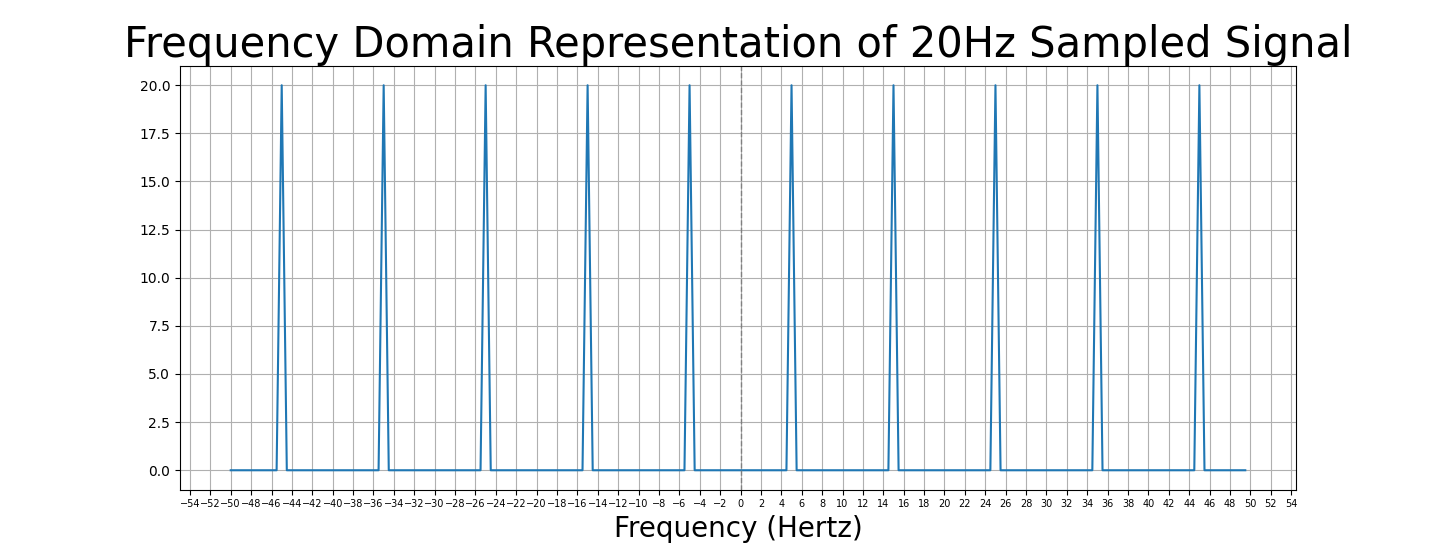
\includegraphics[width=\linewidth]{images/freqdom_20hz.png}
%        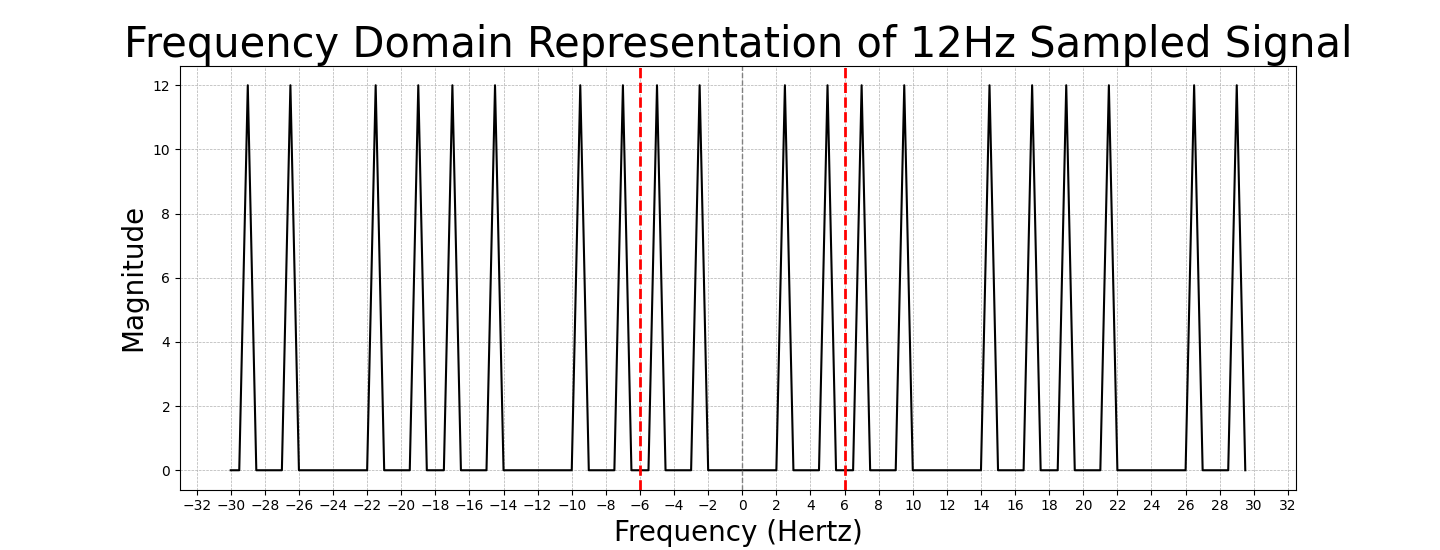
\includegraphics[width=\linewidth]{images/freqdom_12hz_multiple.png}
%        \\[0.5em] 
%    \end{minipage}
    
%    \begin{minipage}{0.5\textwidth}
%        \centering
%        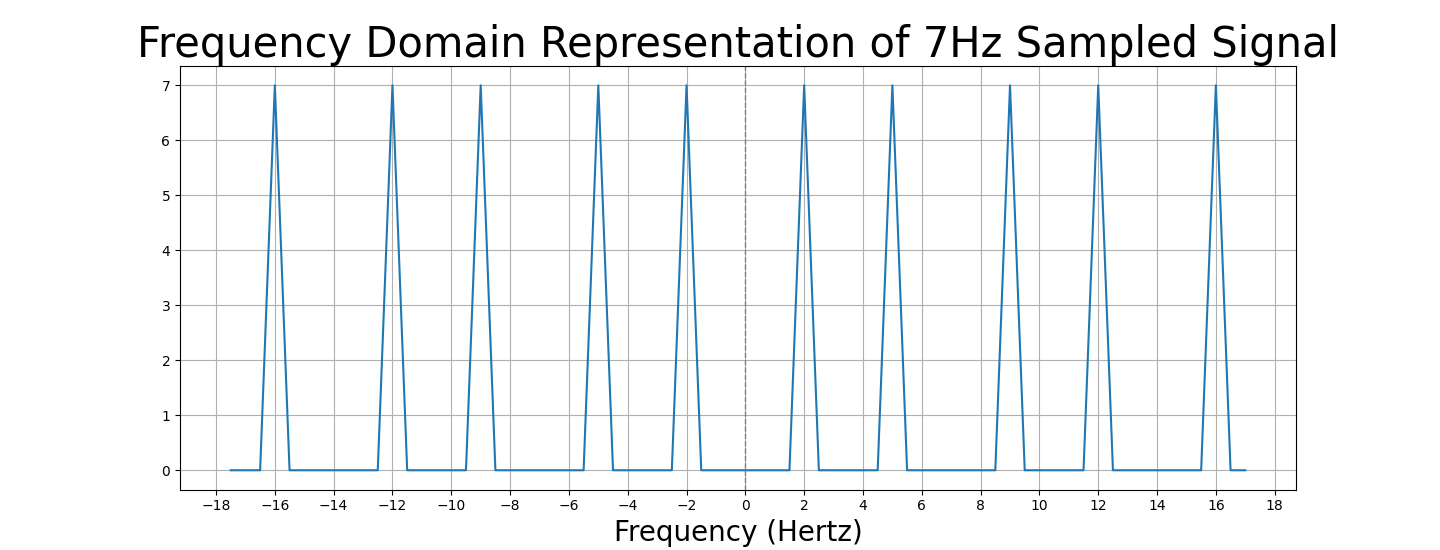
\includegraphics[width=\linewidth]{images/freqdom_7hz.png}
%        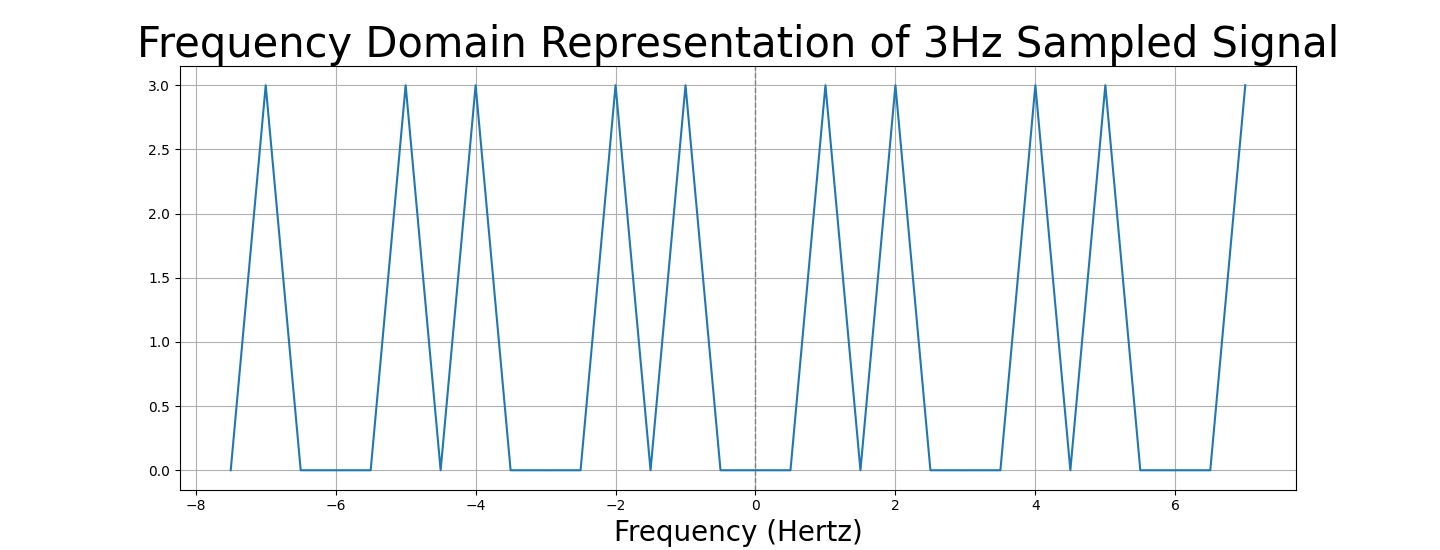
\includegraphics[width=\linewidth]{images/freqdom_3hz.png}
%    \end{minipage}
    
%    \caption{Frequency domain representation of sampled signal at different sampling rates.}
%\end{figure}

%We can observe that the higher the sampling frequency, the 
%When the sampling frequency is above the Shannon-Nyquist threshold, the frequencies closest to 0 are -5 and 5 Hz, which is the true frequency of the original signal (). %insert label of plot here, e.g. top right). 
%However, when the sampling frequency is below this threshold, the frequencies closest to 0 are no longer -5 and 5 Hz. 
%For example, in the plot of sampling frequency 7 Hz (), we see that the frequencies closest to 0 are 2 and -2, and in the plot of sampling frequency 3 Hz (), we see they are 1 and -1 Hz. 
%This becomes an issue when a filter is applied to recover the original signal. 
%give explanation 

%maybe it could be useful to somewhere have like when u use 7hz u could actually construct multiple sine waves that pass through the points. could u code this?

\section{Conclusion}
%maybe link to why this is important if this sine wave wasnt just this arbitrary sine wave but rather an actual signal that needed to be transmitted/used
Through this project, we explored the impact of sampling a time continuous signal above and below the Nyquist rate on signal reconstruction.
%maybe say smth like this is j a toy example so IRL it would be harder to do smth

\begin{thebibliography}{9}
    \bibitem{citekey} Fiveable. ``Signal Digitization -- Biomedical Engineering II." Edited by Becky Bahr, Fiveable, 2024, https://fiveable.me/key-terms/biomedical-engineering-ii/signal-digitization. Accessed 22 Apr. 2025.
    \bibitem{citekey} MacLeod, Cameron. “Fourier Transforms with Scipy.Fft: Python Signal Processing.” Real Python, Real Python, 1 Sept. 2022, realpython.com/python-scipy-fft/. Accessed 13 Apr. 2025. 
\end{thebibliography}

%np.interp: https://numpy.org/doc/2.1/reference/generated/numpy.interp.html

\section{Appendix}
\begin{enumerate}
    \item Access the GitHub repository with all code \href{https://github.com/margheritatonon/approximation-II-assignment}{here}.
\end{enumerate}




\end{document}
